
\documentclass[12pt, letterpaper]{article}
\title{Lab Report C2}
\usepackage{graphicx}
\usepackage{amsmath}
\usepackage[margin=1in]{geometry}% Sets 1in margins. 
\usepackage{fancyhdr}			% Creates headers and footers
\usepackage{enumerate}    
\usepackage{booktabs, multirow}%These two package give custom labels to
\usepackage[shortlabels]{enumitem}
\author{Aditya Gupta}
\date{\today}
\begin{document}
\maketitle
\newpage
\tableofcontents
\newpage
\section{Graph of Terminal Velocity vs Mass}
\begin{table}[!htp]\centering
\scriptsize
\begin{tabular}{lrrr}\toprule
Mass(g) &Terminal Velocity(cm/s) &uncertainty of terminal velocity \\\midrule
0.9 &87.91 &79.12 \\
1.5 &119.76 &179.64 \\
2.1 &150.37 &315.79 \\
2.7 &156.25 &421.87 \\
3.3 &197.05 &650.25 \\
3.9 &199.04 &776.12 \\
\bottomrule
\end{tabular}
\end{table}
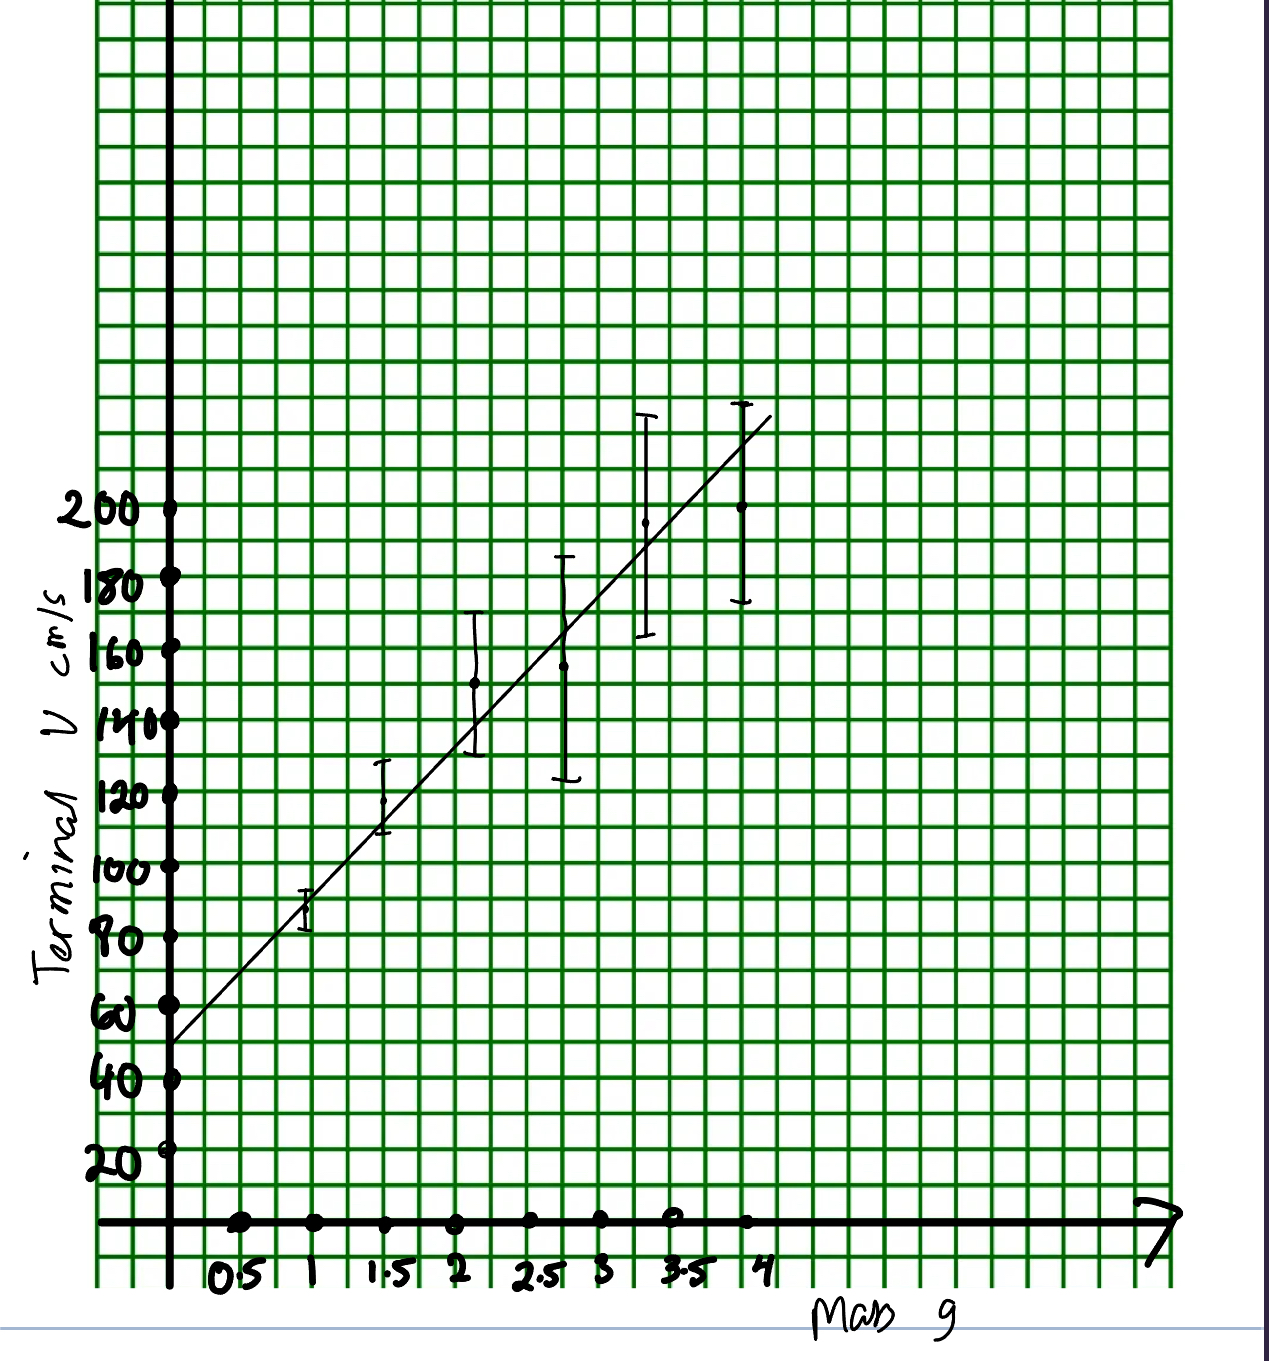
\includegraphics[width=1\linewidth]{printable-quarter_inch_green_graph_paper-4x.jpeg}

Line of best fit:
\[
tv(m) = 40.7m + 50
\]

\section{Graph of Square of Terminal Velocity vs Mass}
\begin{table}[!htp]\centering
\scriptsize
\begin{tabular}{lrrr}\toprule
Mass(g) &Square of terminal velocity &uncertainty in square of terminal velocity \\\midrule
0.9 &7728.54 &1058.58 \\
1.5 &14342.57 &2621.91 \\
2.1 &22612.92 &7205.40 \\
2.7 &24414.06 &9234.40 \\
3.3 &38826.47 &11000.56 \\
3.9 &39602.98 &11110.80 \\
\bottomrule
\end{tabular}
\end{table}
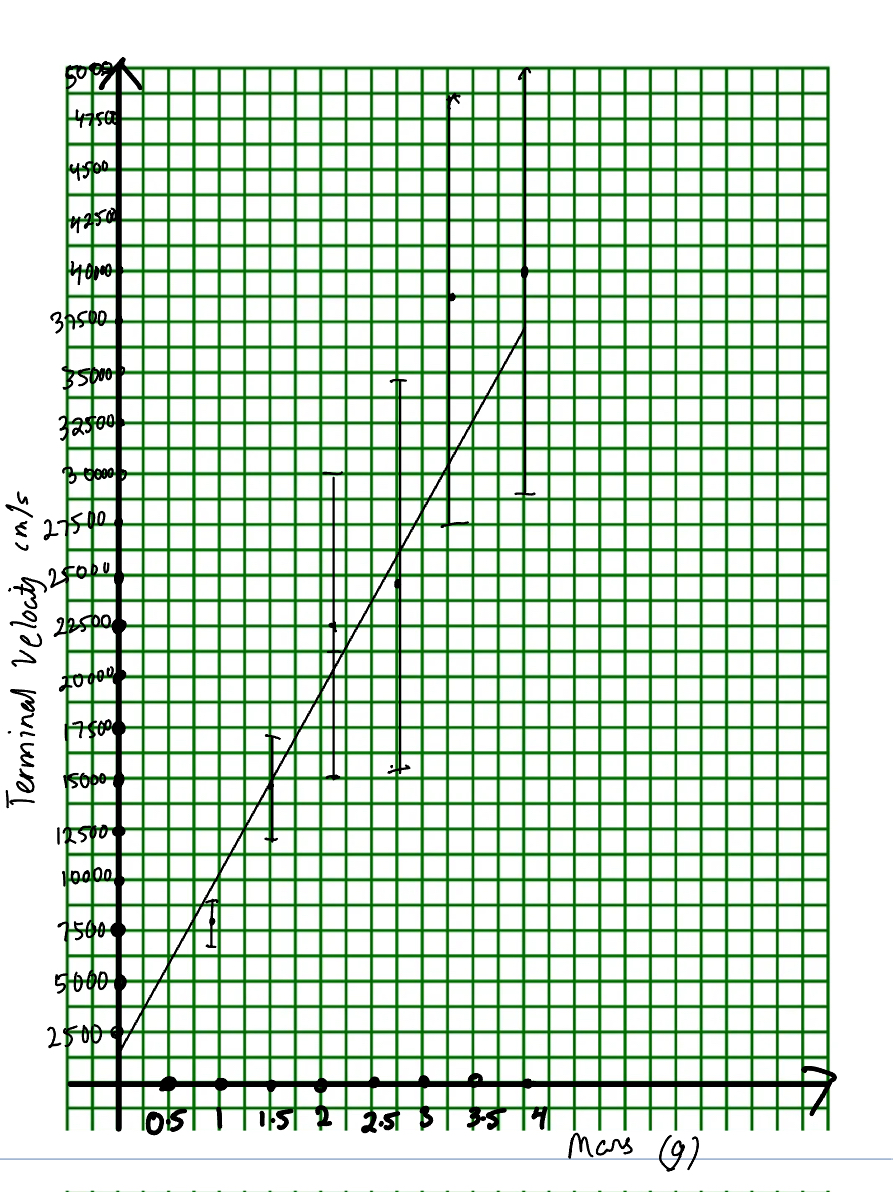
\includegraphics[width=0.6\linewidth]{printable-quarter_inch_green_graph_paper-4x Copy.jpeg}

Line of best fit:

\[
tv^2(m) = 9090x + 1250
\]

\section{Conclusion}

The goal of this experiment was to determine which of two models from Section 2.1 best describes the relationship between terminal speed ($v_t$) and mass ($m$) for objects in free fall.

The first graph, $v_t$ versus $m$, yielded a best-fit line of $v_t = 40.7m + 50$. The relatively large $y$-intercept of 50 suggests that for small masses, the model may deviate from theoretical predictions. This could indicate that terminal speed does not increase proportionally with mass for lower values.

The second graph, $v_t^2$ versus $m$, produced a best-fit line of $v_t^2 = 9090m + 1250$. While the $y$-intercept is still present, it is relatively smaller compared to the first graph when considering the scale of the data. This smaller $y$-intercept indicates that the squared terminal speed model has less offset and aligns better with the expected trends for terminal velocity as a function of mass.

Based on these observations, the squared terminal velocity model better fits the data. The smaller $y$-intercept suggests a closer alignment with theoretical expectations, making this model the most consistent with the evidence collected during the experiment.

\end{document}